\documentclass[border=3mm,multi=tikzpicture]{standalone}
\usepackage{pgfplots}\pgfplotsset{compat=1.18}
\usepackage[european,straightvoltages]{circuitikz}
\usepackage{fontspec}\setmainfont{Liberation Sans}
\usepackage{unicode-math}\setmathfont{TeX Gyre DejaVu Math}\newcommand{\Ohm}{Ω}
\definecolor{dunkel}{HTML}{1F3A5F}\definecolor{rot}{HTML}{C62828}
\begin{document}
% 1 Kennlinie neutral
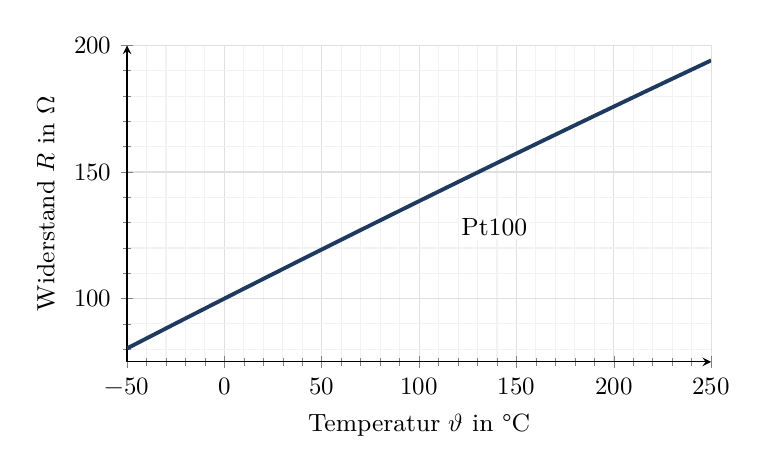
\begin{tikzpicture}
\begin{axis}[width=9cm,height=5.6cm,xmin=-50,xmax=250,ymin=75,ymax=200,
  xlabel={Temperatur $\vartheta$ in °C},ylabel={Widerstand $R$ in \Ohm},
  grid=both,grid style={black!12},minor tick num=4,minor grid style={black!5},axis lines=left,
  /pgf/number format/use comma,every axis label/.style={font=\small},tick label style={font=\small}]
\addplot[dunkel,line width=1.4pt,domain=-50:250,samples=60] {100*(1+0.0039083*x-0.0000005775*x^2)};
\node[font=\small,fill=white,inner sep=1pt,anchor=west] at (axis cs:120,128) {Pt100};
\end{axis}
\end{tikzpicture}
% 2 Zwei-, Drei-, Vierleiter allgemein
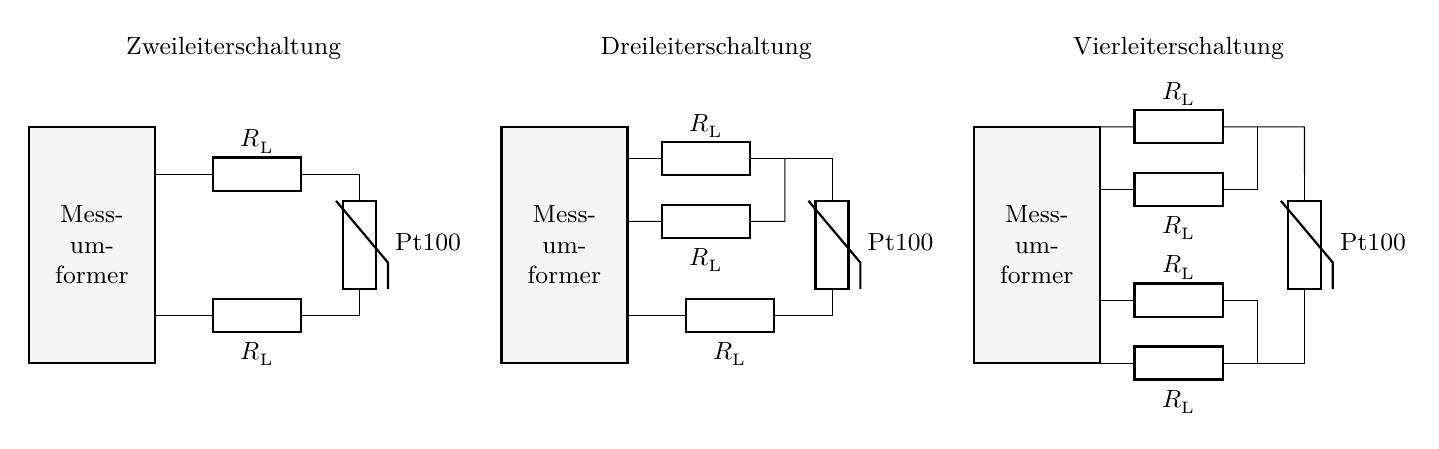
\begin{tikzpicture}[font=\small]
\foreach \x/\n/\t in {0/2/Zweileiterschaltung,6/3/Dreileiterschaltung,12/4/Vierleiterschaltung}{
 \begin{scope}[xshift=\x cm]
 \draw[line width=0.9pt,fill=black!4] (0,0) rectangle (1.6,3) node[midway,align=center]{Mess-\\um-\\former};
 \node at (2.6,4.0) {\t};
 \draw (4.2,0.6) to[thR,l_=Pt100] (4.2,2.4);
 \ifnum\n=2
  \draw (1.6,2.4) to[R,l=$R_\mathrm{L}$] (4.2,2.4); \draw (1.6,0.6) to[R,l_=$R_\mathrm{L}$] (4.2,0.6);
 \fi
 \ifnum\n=3
  \draw (1.6,2.6) to[R,l=$R_\mathrm{L}$] (3.6,2.6) -| (4.2,2.4); \draw (1.6,1.8) to[R,l_=$R_\mathrm{L}$] (3.6,1.8) -- (3.6,2.6);
  \draw (1.6,0.6) to[R,l_=$R_\mathrm{L}$] (4.2,0.6);
 \fi
 \ifnum\n=4
  \draw (1.6,3.0) to[R,l=$R_\mathrm{L}$] (3.6,3.0) -| (4.2,2.4); \draw (1.6,2.2) to[R,l_=$R_\mathrm{L}$] (3.6,2.2) -- (3.6,3.0);
  \draw (1.6,0.8) to[R,l=$R_\mathrm{L}$] (3.6,0.8) -- (3.6,0.0); \draw (1.6,0.0) to[R,l_=$R_\mathrm{L}$] (3.6,0.0) -| (4.2,0.6);
 \fi
 \end{scope}}
\end{tikzpicture}
% 3 Anschlussbild Datenblatt (Aderfarben nach IEC 60751)
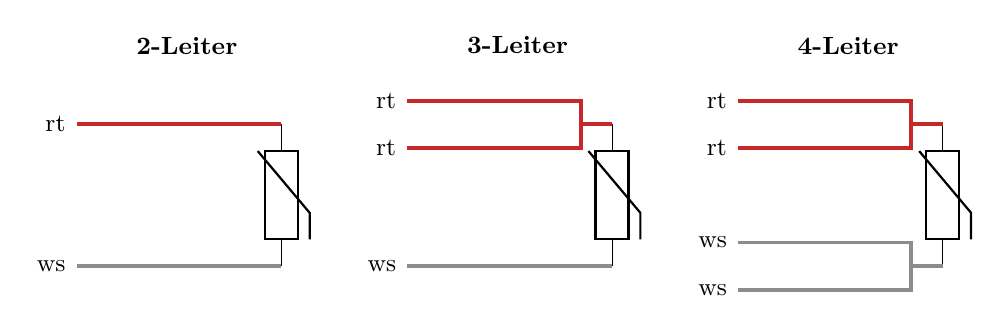
\begin{tikzpicture}[font=\small]
\foreach \x/\n/\t in {0/2/2-Leiter,4.2/3/3-Leiter,8.4/4/4-Leiter}{
 \begin{scope}[xshift=\x cm]
 \node[font=\small\bfseries] at (1.4,3.4) {\t};
 \draw (2.6,0.6) to[thR] (2.6,2.4);
 \ifnum\n=2 \draw[rot,line width=1.4pt] (0,2.4) node[left,black]{rt} -- (2.6,2.4); \draw[black!45,line width=1.4pt] (0,0.6) node[left,black]{ws} -- (2.6,0.6); \fi
 \ifnum\n=3 \draw[rot,line width=1.4pt] (0,2.7) node[left,black]{rt} -| (2.2,2.4) -- (2.6,2.4); \draw[rot,line width=1.4pt] (0,2.1) node[left,black]{rt} -- (2.2,2.1) -- (2.2,2.4);
   \draw[black!45,line width=1.4pt] (0,0.6) node[left,black]{ws} -- (2.6,0.6); \fi
 \ifnum\n=4 \draw[rot,line width=1.4pt] (0,2.7) node[left,black]{rt} -| (2.2,2.4) -- (2.6,2.4); \draw[rot,line width=1.4pt] (0,2.1) node[left,black]{rt} -- (2.2,2.1) -- (2.2,2.4);
   \draw[black!45,line width=1.4pt] (0,0.9) node[left,black]{ws} -- (2.2,0.9) |- (2.6,0.6); \draw[black!45,line width=1.4pt] (0,0.3) node[left,black]{ws} -- (2.2,0.3) -- (2.2,0.6); \fi
 \end{scope}}
\end{tikzpicture}
\end{document}
